\chapter{Parameter Estimation Methodologies}
\label{chap:paramest}

Below are the various different methods for parameter estimation that I investigated during the course of this work. All of these methods involve a sampling system that attempts to select parameter values which minimise the difference between the simulation result and the experimental data by calculating a \textit{fitness value}. The aim of the parameter estimation methodology was to get this \textit{fitness value} as close to zero (perfect fit/no difference) as possible. Two different calculations were used to create the \textit{fitness value}. One was the sum of the Least Squares Differences between the measured components in the experimental data and the simulation result. This was used in early parameter estimation runs.

\begin{equation}
f = \sum^{n}_{j=1}\left(\sqrt{\sum^{m}_{i=1} (\Delta x_{ij})^2}\right)
\end{equation}

The second method for calculating the \textit{fitness value} was a lognormal correlation which allowed greater tuning, as the standard deviation of the distribution could be set to adjust how much fitter the simulation result needed to be to be accepted.

\begin{equation}
f = \sum^{n}_{j=1}\left(\sum^{m}_{i=1}\left(\ln\left(\dfrac{1}{2\pi\sigma_j^2}e^{-\dfrac{{(0-0)^2}}{2\sigma_j^2}}\right) - \ln\left(\dfrac{1}{2\pi\sigma_j^2}e^{-\dfrac{{(x_{ijFIT}-x_{ijDATA})^2}}{2\sigma_j^2}}\right)\right)\right)
\end{equation}

In most cases the components used for calculating the \textit{fitness value} are Oxygen and Nitric Oxide, as these were the primary measured chemicals.

The main difference between the parameter estimation methodologies laid out below are the ways in which they generate new parameter values, either from a probability distribution or based on the previous value, and the way this is applied and tested against the experimental data.

\section*{Monte Carlo Methods}

I include a brief section here to describe Monte Carlo Methods, as the techniques I used for parameter estimation all use this method as their estimator in some form.
``Monte Carlo Methods'' is a generalised term to describe a stochastic technique that makes use of random numbers to examine a problem in conjunction with probability statistics. Monte Carlo Methods allow us to model complex systems without having to exhaustively search every possible outcome. Large systems are sampled in random configurations and that data applied in such a way that it can be used to describe the system as a whole. ``Monte Carlo techniques are often the only practical way to evaluate difficult integrals or to sample random variables governed by complicated probability density functions''\cite{Nakamura2010}.

\section{Simulated Annealing}

This technique was described independently by \citet{Kirkpatrick1983} and \citet{Cerny1985}. The name comes from the metallurgical annealing process whereby large crystals are formed while a material is slowly cooled. The slow cooling increases the probability of individual crystals obtaining lower energy states than the initial. As the material cools the ``distance'' each crystal can move along the energy landscape decreases.
\citet{Bertsimas1993}

The algorithm used to modify the parameter sets is broadly based on simulated annealing in addition to a simple genetic algorithm.
 
In this scheme a synthetic ``chromosome'' is created containing ``genes'' which represent parameters in the simulation. These include the rate constants, concentrations of various components and initial concentrations of substrates and products. The initial parameter set is loaded onto the chromosome and those parameters are used to solve the sets of differential equations as above. This generates data at time points (every 0.001s) during the simulation which can be plotted and compared against known experimental values. By calculating the least-squares-difference between the result from the simulation, and the experimental data, it is possible to generate an ``unfitness'' value for the simulated data. This is a representation of how close the simulated data is to the experimental data, an unfitness value of 0 being a perfect fit. 

The genetic algorithm is then used to improve these parameters by mutating genes (individual parameters) from fit chromosomes (complete parameter sets), re-running the simulation and discarding unfit parameter sets. An unfit parameter set is defined as one with an unfitness value lower than the best so far. This technique involves having two chromosomes selected at any one time. The parameters from each chromosome are simulated and the least fit one is discarded. At this point the contents from the fitter chromosome are cloned and mutated, and the cycle is repeated.

\begin{figure}
	\begin{center}
		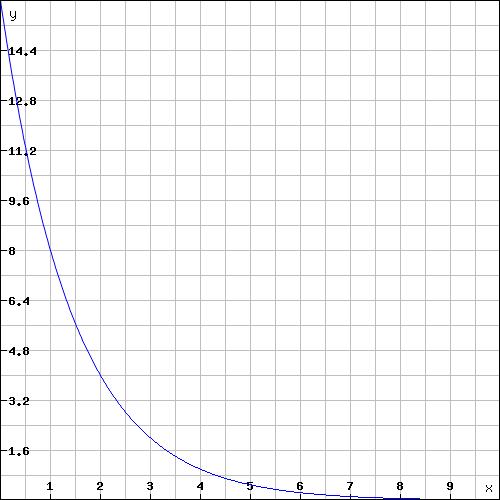
\includegraphics[height=10cm]{03-parameterestimationmethodologies/data/temperature.png}
		%a0=2&a1=1/((2^x)/16)&a2=&a3=&a4=1&a5=4&a6=8&a7=&a8=1&a9=1&b0=500&b1=500&b2=0&b3=10&b4=0&b5=16&b6=10&b7=10&b8=5&b9=5&c0=3&c1=0&c2=1&c3=1&c4=1&c5=1&c6=1&c7=0&c8=0&c9=0&d0=1&d1=20&d2=20&d3=0&d4=&d5=&d6=&d7=&d8=&d9=&e0=&e1=&e2=&e3=&e4=14&e5=14&e6=13&e7=12&e8=0&e9=0&f0=0&f1=1&f2=1&f3=0&f4=0&f5=&f6=&f7=&f8=&f9=&g0=&g1=1&g2=1&g3=0&g4=0&g5=0&g6=Y&g7=ffffff&g8=a0b0c0&g9=6080a0&h0=1&z
	\caption[Example simulated annealing temperature schedule]{{\bf Example simulated annealing temperature schedule.} This represents how the annealing temperature changes as the annealing process progresses. Temperature is denoted by the y-axis value, and simulation progress by the x-axis value. This is a heavily compressed timeframe, as in reality the system would normally process 10,000 sets of parameters at each annealing temperature.
	\label{fig:temperature}}
	\end{center}
\end{figure}


As part of the simulated annealing algorithm, an ``annealing temperature'' is set. The value defines how large a change the mutation can effect on a particular gene. Since all the parameters are numerical values, this value could be used to define that a mutation can only alter the value by a maximum of 10\%. This value is programmed to decrease after a defined number of iterations such that the magnitude of individual mutations becomes smaller as the simulation progresses. This should have the effect of honing in on a set of parameters with high fitness.

\begin{figure}
\begin{verbatim}
c1 <- c0;
c2 <- mutate(c1);
i <- 0;
while i < i_max
  if fitness(c1) > fitness(c2)
    c2 <- mutate(c1)
  else
    c1 <- mutate(c2)
  i <- i + 1
if fitness(c1) > fitness(c2)
  return c1
else
  return c2
\end{verbatim}
\caption[Pseudo-code showing how the simplest annealing algorithm works.]{{\bf Pseudo-code showing how the simplest annealing algorithm works.}
\label{fig:sa_code}}
\end{figure}

Figure~\ref{fig:sa_code} contains some simple pseudo-code which shows how the basic algorithm works (without the annealing temperature). This will provide a ``best'' parameter set, but there is no information about the possible spread of values in the parameter set. To access this information, the annealing technique has to be altered to allow a pool of chromosomes to be used. In this scenario a large (30, currently) pool of chromosomes are created from the initial parameter set and then 2
are chosen at random from the pool. The basic simulation process continues as above, with the fitness of both parameter sets being compared, and the least fit parameter set being replaced with a mutation of the fitter set. At this point both chromosomes are returned to the pool and 2 new chromosomes are chosen at random from the pool. After a large number of iterations (1000's), the pool should contain chromosomes all with good fitness values, from which it is possible to calculate the spread of parameters. Figure~\ref{fig:sa_spread} shows this diagrammatically. The spread of the parameters can be used to infer the sensitivity of the simulation to changes in parameter values in a similar way to that described by \citet{Toni2009}.

The algorithm currently used also includes a gene mask in the chromosome which allows any number of genes to be switched on or off. In this way it is possible to fix the values of certain parameters, and prevent them from being mutated at each iteration. This is useful during the parameter search process, as a limited dataset can be used, which only describes a limited subset of the overall model, and any parameters which are unrelated to that dataset can be removed. Practically this means it is possible to focus on one particular aspect of the model, such as oxygen utilisation, set all the parameters which are irrelevant to zero, and prevent them from being included in the genetic algorithm. During this process, the parameters related to oxygen utilisation can be improved, and once a sufficient set of value is obtained, these can then be fixed when a different dataset is used, such as \cNO \space reduction.

\begin{figure}
\begin{center}
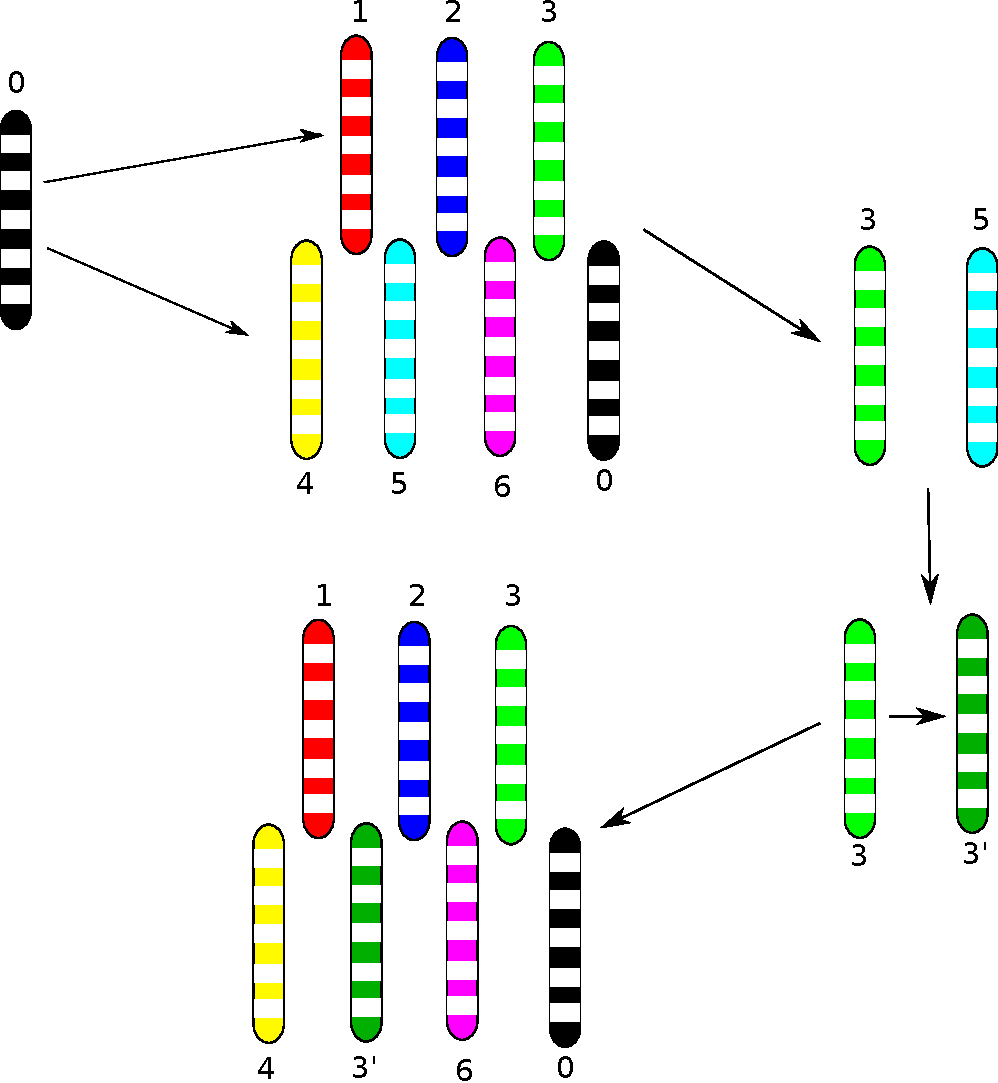
\includegraphics[height=10cm]{./03-parameterestimationmethodologies/data/sa_spread.pdf}
% sa_spread.pdf: 479x520 pixel, 72dpi, 16.90x18.34 cm, bb=0 0 479 520
\end{center}
\caption[{Schematic diagram showing the technique used to generate a spread of parameters using a synthetic chromosome.}]{{\bf Schematic diagram showing the technique used to generate a spread of parameters using a synthetic chromosome.} The parameters are loaded as genes on the chromosome which are then mutated, 2 chosen and the fittest kept and mutated. Each time a chromosome is mutated it is reintroduced into the chromosome pool, and the next 2 chromosomes are chosen at random.
\label{fig:sa_spread}}
\end{figure} 





\section{Approximate Bayesian Computation by Sequential Monte Carlo}

To incrementally improve the parameter sets, a version of bayesian inference is used in conjunction with a standard monte-carlo method in a system called Approximate Bayesian Computation by Sequential Monte Carlo (ABCSMC) as described by \citet{Toni2009}. Algorithm (S) was used from that paper.

\textit{Bayesian Inference} - This a statistical method for inferring the probability of a hypothesis based on available evidence. As more evidence is accumulated, the inference is updated and the probability of the hypothesis being true is changed. Given enough evidence, the probability of the hypothesis being true should either be very high or very low causing you to either accept or reject the hypothesis. Bayesian inference relies on having a prior probability (or probability distribution) for the hypothesis, and this can inevitably introduce a level of bias into the inference.

\textit{Approximate Bayesian Computation} - This is an adaptation of bayesian inference which allows approximately the same inferences to be made, with considerably less computation. It operates on representations of the datasets rather than the datasets themselves. Common examples are population mean and variance. This is useful for large complex datasets where the probability of a simulation of the dataset matching the original is very small (unacceptably so), in this case a representation of the datasets can be used, and the difference calculated. If the difference is less than a pre-defined acceptance threshold, then the simulated dataset is accepted.

\textit{Sequential Monte Carlo} - This is a method of particle filtering whereby a large set of samples ($N$) are drawn from the prior distribution, and for each sample, the probability is calculated. Weights for each particle are assigned based on the probabilities, and these affect how likely a particle is to be selected in subsquent rounds of selection. At the end of each round, the posterior distribution, that of the $N$ particles becomes the prior distribution for the next round.

\textit{Approximate Bayesian Computation by Sequential Monte Carlo} - This combines the previous two methods by drawing a large number of particles from the prior distribution using bayesian inference. The prior distribution is discrete in the scheme used here, so a perturbation kernel based on a laplacian or gaussian distribution is used on each sample to provide small deviations to better approximate a continuous prior distribution. Each sample is simulated and only accepted if it exceeds the acceptance theshold. This is calculated based on the least-sequares difference (LSD) between the simulated data and the original dataset. If a sample is rejected, a new one is drawn from the prior distribution and SMC then continues as described above. The weights of the accepted samples are calculated based on the probabilities of being selected from the prior and the samples go on to form the posterior distribution. For each subsequent round, the mean LSD of the posterior distribution from the previous round is used as the acceptance threshold. This ensures that each round results in better fitting parameter sets. The cycle is then repeated until a pre-defined cycle limit is reached \cite{Toni2009}.

A significant advantage of this technique is that it is readily parallelisable, as each particle in the SMC process is independent, thus can be simulated in parallel. A parallel version of this algorithm has been implemented in the java programming language which results in significant speedups when multiple processing threads can be used. The threading manager means that the algorithm is theoretically most efficient (in terms of computational time) when the number of particles is an exact multiple of the number of processing threads. In practice however this is negated by the fact that some particles require multiple samples due to them not meeting the acceptance criteria.


\section{Metropolis Hastings Monte Carlo}

The Metropolis-Hastings algorithm is Markov Chain Monte Carlo method to retrieve sequences of random samples from a probability distribution which cannot be sampled directly (or would be very difficult) such as when no probability distribution function exists. The algorithm was originally developed by \citet{Metropolis1953} for generating samples from the boltzman distribution. It was later extended to a more general form for any distribution by \citet{Hastings1970}.

MHMC allows each individual parameter to follow a biased random walk until it reaches a point of maximum ``fitness.'' The typical output of this algorithm is a set of parameter trajectories which begin with a ``burn in'' period, followed by a parameter distribution. The ``burn in'' period contains data that is discarded, as it does not form part of the target distribution. The length of this burn in period often varies depending on how far the starting samples are from the target distribution. The parameter distribution can be calculated from the data that is left after the burn in period. This is done by a simple statistical analysis of the resulting data points. Since the distributions cannot easily be described as functions, the data are transformed into histograms with a set bin width. These histograms can be read and used a priors for subsequent runs of the MHMC algorithm.

The MHMC algorithm has been validated initially by using a much simpler ODE system than is required by the respiration model. A Lotka-Volterra system was used as this can be solved much more quickly by virtue of having far fewer parameters (4 as opposed to \gt 20). The Lotka-Volterra system describes a simple predator-prey relationship and only requires two first-order, non-linear differential equations, which are shown in equation \ref{eq:lv}.

\begin{eqnarray}
\frac{dx}{dt} = x (\alpha - \beta y)\nonumber \\
\frac{dy}{dt} = -y (\gamma - \delta x)
\label{eq:lv}
\end{eqnarray}

Validation of using this system required a simulated dataset with known parameter values to be produced. This dataset then forms the input for the MHMC algorithm which will try and obtain those same parameter values. Given the simplicity of this system, a particularly bad set of initial parameter estimates was given to exaggerate the burn in period, and to show that given a long enough time the simulation will eventually settle on ``correct'' values. This validation step also informs the likely values for two tuning variables in the algorithm; the \textit{acceptance} - how stringent the algorithm is on accepting new parameter sets, and the \textit{sigma} value - this describes the magnitude of parameter perturbation at each iteration.
The graphical results of the Lotka-Volterra validation are shown in figures \ref{fig:simulation} and \ref{fig:parameters}.

\begin{figure}
 \centering
 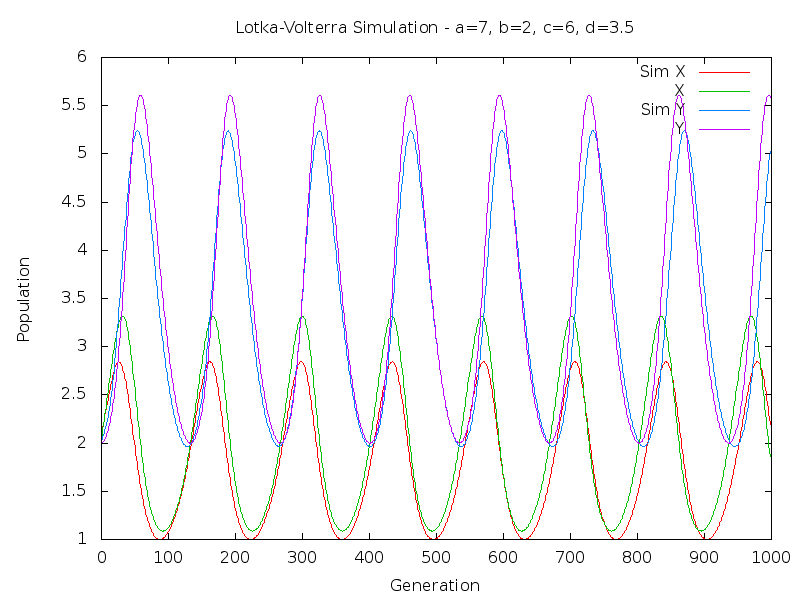
\includegraphics[width=14cm]{./03-parameterestimationmethodologies/data/Simulation.png}
 % Simulation.png: 800x600 pixel, 72dpi, 28.22x21.17 cm, bb=0 0 800 600
 \caption[{Simulation results of the Lotka-Volterra validation run.}]{{\bf Simulation results of the Lotka-Volterra validation run.}
 \label{fig:simulation}}

\end{figure}

\begin{figure}
 \centering
 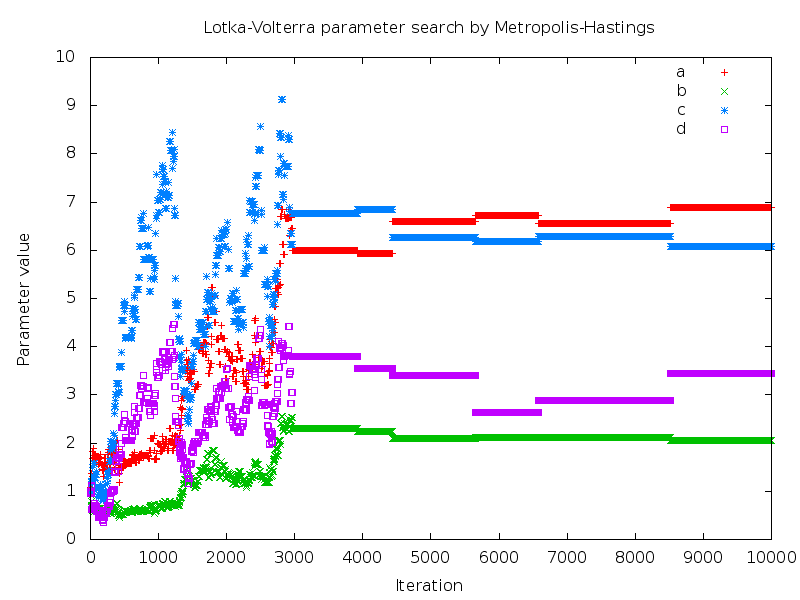
\includegraphics[width=14cm]{./03-parameterestimationmethodologies/data/Parameters.png}
 % Simulation.png: 800x600 pixel, 72dpi, 28.22x21.17 cm, bb=0 0 800 600
 \caption[{MHMC results of the Lotka-Volterra validation run.}]{{\bf MHMC results of the Lotka-Volterra validation run.} Note the initial burn-in period followed by the distribution trajectory.
 \label{fig:parameters}}
\end{figure}

\section{Implementation}
The initial parameters used to solve the equations were a set of priors based on preliminary experimental results. These parameters only provide a starting point as the second stage of computation involves modifying the parameters in order to provide a better fit against experimental data. To incrementally improve the parameter sets, a version of Bayesian inference is used in conjunction with a standard Metropolis-Hastings Monte-Carlo method.

We used Bayesian inference to inform the simulation parameters for a particular dataset based on prior probability distributions. These distributions were obtained as output from a previous dataset. We integrated this with a Metropolis-Hastings algorithm for sampling the prior probability distributions. Each parameter was sampled, and the parameter set was used to solve the ODE model. Based on the fitness output of the solved model, the Metropolis-Hastings algorithm allows parameters to be modified in a biased random walk which ultimately leads them to their most fit state, calculated using Least Squared Difference.

\section{Integrative Scheme}
In order for us to iteratively generate a parameter set we needed to separate the model into simpler units whereby we can obtain data about a specific set of variables. We did this so that the simplest part of the model was parametrised first. In this case it was oxygen respiration, which only requires one enzyme (although it does still require the electron transport chain). This section of the model also has the simplest experimental dataset. After parametrisation, a new section of the model was introduced, with its associated experimental dataset.

Experimental data was gathered for the first dataset, and this is used as a training set, with almost flat priors based on preliminary experimental data. The data was pre-processed and normalised if necessary and then presented to the Bayesian Parameter Estimation system. The MHMC algorithm samples from the prior distribution and then uses those samples as parameters to solve the model. It aims to improve the calculated fitness value and is ordinarily run for at least 100,000 iterations to give the system time to settle on the fittest parameters. The system is run on the same dataset 10 times to generate statistically significant results. The eventual output of the MHMC runs are posterior probability distributions for each of the parameters in the model. In accordance with Bayesian inference these are then used as prior distributions.

At this point the next section of the model to be parametrised is decided, the appropriate experimental data identified and obtained, and the process is repeated until the entire model has been populated. The final result should be a set of reasonably narrow probability distributions for each of the parameters which describe the system accurately enough to correctly predict the behaviour of the system \textit{in vivo}.